\section{Modern GPGPUs}

This section will cover recent developments in GPGPUs.

\subsection{Reality of Warps}

Recall the Fermi SM diagram in Figure \ref{fig:fermiSM}.
We have two sets of 16 SPs corresponding
two two warp schedulers, giving us 16 SPs per warp.

Imagining warps as 32 cores executing in lock-step is useful in explaining things,
but it isn't realistic. In reality, warp execution takes two cycles as shown
in Figure \ref{fig:exec}. The part on the bottom shows the execution steps
of instructions 0, 1, and 2 shown on the top part \cite{yt}.

\begin{figure}[h]
    \centering
    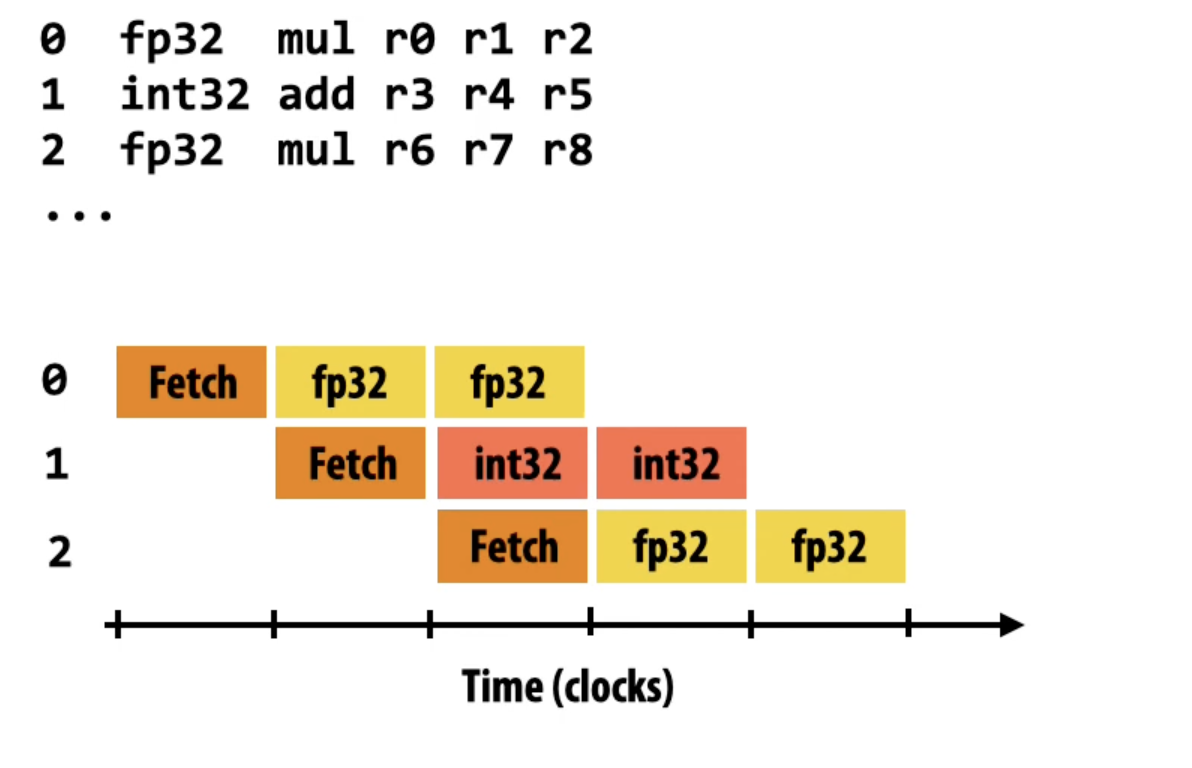
\includegraphics[width=0.5\textwidth]{assets/execex.png}
    \caption{Example of execution of 32 thread warps on 16 SPs.}
    \label{fig:exec}
\end{figure}

\subsection{Recent Developments}

\textbf{Kepler:} This is the first Nvidia GPU to introduce a compiler generate control instruction.
This is inserted every 7 instructions. One byte of the 64-bit instruction indicates
that this is a control instruction. The other 7 bytes encode information for the
next 7 instructions \cite{chipsandcheeseInsideKepler}.

This control instruction encodes latency information, preventing write-after-read hazards
from occuring between fixed-latency instructions \cite{chipsandcheeseInsideKepler}.

These instructions still modify a central scoreboard that the scheduler that
issues instructions looks to \cite{chipsandcheeseInsideKepler} \cite{adalbert2022pastis}.

In addition, these instructions encode whether or not instructions can be dual-issued \cite{chipsandcheeseInsideKepler}.

\textbf{Maxwell:} This architecture increases the frequency of the control word,
inserting it every 3 instructions instead of every 7. 

Maxwell control instructions include information pertaining to variable latency
instructions. This works by assigning destination registers of these instructions
to a barrier in hardware. Instructions that then have those
registers as operands must wait until the barriers clear up. This means
that Maxwell needs less scoreboarding hardware \cite{chipsandcheeseMaxwellNvidias}.

A one-bit yield flag is also introduced in this architecture. This instructs
the scheduler to prefer to switch execution to another warp instead of continuing
instructions from a single warp (\cite{githubControlCodes}, \cite{jia2018dissecting}). 
The hardware still makes most scheduling decisions on its own but there are
situations where this bit can lead to performance improvements \cite{githubControlCodes}.

This architecture also introduced an operand reuse cache \cite{chipsandcheeseMaxwellNvidias}. 
In this architecture, registers are assigned to banks naively (register number modulo 4, the number of banks).
What allows this to work is the reuse cache. The cache has entries for 4 operands.
When an issuing an instruction, a hardware unit checks the corresponding part of the control instruction
to see whether or not flags indicating that some registers will be used again are set.
If so, it can save those registers in the reuse cache. Future uses of those
registers in the same operand slot can access the value from the reuse cache,
avoiding having to access the register file, reducing bank conflicts (\cite{jia2018dissecting}, \cite{githubSGEMM}, \cite{chipsandcheeseMaxwellNvidias}).

\textbf{Volta:} Volta increases the instruction word from 64 bits to 128 bits.
It also starts to include control information within instructions instead of
using a control word\cite{jia2018dissecting}.

This architecture also introduces the Tensor Core \cite{sun2022dissecting}.

Volta also replaces the SIMT Stack based handling of warp divergence with
barriers \cite{aamodt2018general}.
